\graphicspath{{lectures/02_eloadas_abrak/}}

\section{Differenciálegyenletek felállítása}

\subsection{Parabolatükör}

Milyen forgásfelület legyen?

\begin{center}
  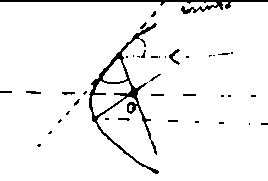
\includegraphics[width=.26\textwidth]{01_parabolatukor_tukor.png}
\end{center}

Legyen $y(x)$ a keresett görbe, $y\in D$, és $y(x)>0$.
A geometriai ábrán $P\bigl(x,y(x)\bigr)$; az érintő és az $x$ tengely
által bezárt szög $\alpha$.

\begin{center}
  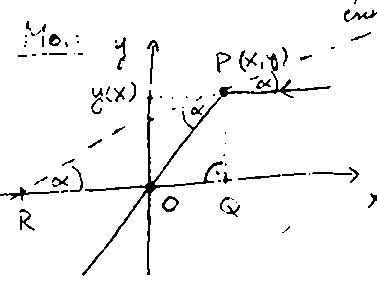
\includegraphics[width=.39\textwidth]{02_parabolatukor_geometria.png}
\end{center}

\[
  |OP|=|OR|=\sqrt{x^2+y^2(x)}.
\]

\[
  \operatorname{tg}\alpha=y'(x)
  =\frac{|QP|}{|RQ|}
  =\frac{y(x)}{x+\sqrt{x^2+y^2(x)}}.
\]

Tehát a felírt differenciálegyenlet:
\[
  \boxed{\displaystyle
  y'(x)=\frac{y(x)}{x+\sqrt{x^2+y^2(x)}}},
  \qquad y(x)>0. \tag{$*$}
\]

\noindent\textbf{Megoldás: gyöktelenítés.}
\begin{align*}
 y'(x)
 &=\frac{y(x)}{x+\sqrt{x^2+y^2(x)}}
   \cdot\frac{x-\sqrt{x^2+y^2(x)}}{x-\sqrt{x^2+y^2(x)}}\\
 &=\frac{y(x)\bigl(x-\sqrt{x^2+y^2(x)}\bigr)}{-y^2(x)}\\
 &=\frac{\sqrt{x^2+y^2(x)}-x}{y(x)}.
\end{align*}

Ebből
\[
 y(x)y'(x)+x=\sqrt{x^2+y^2(x)}.
\]

Az $x^2+y^2(x)$ kifejezés deriváltját felhasználva:
\[
 \bigl(x^2+y^2(x)\bigr)'=2\sqrt{x^2+y^2(x)}.
\]

Jelölje $F(x)=x^2+y^2(x)$. Ekkor
\[
  F'(x)=2\sqrt{F(x)},
\]
\[
  F(x)=(x-c)^2=x^2+y^2(x)
  \quad\Longrightarrow\quad
  \boxed{y^2(x)=-2xc+c^2}.
\]

Ez a \textbf{parabola egyenlete}.

\subsection{Láncgörbe}

A láncgörbe a hiperbolikus koszinusz, $\operatorname{ch}(x)$ képével írható le.
Két végén rögzített lánc egyensúlyi helyzetben felvett alakja:
az $y(x)$ görbe.

\begin{center}
  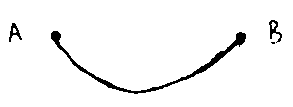
\includegraphics[width=.30\textwidth]{03_lancgorbe.png}
\end{center}

Fizikai megfontolások alapján igazolható:
\[
  \boxed{y''(x)=\frac{\gamma}{H}\sqrt{1+\bigl(y'(x)\bigr)^2}}.
\]

Legyen $u=y'$. Ekkor
\[
  u'(x)=\frac{\gamma}{H}\sqrt{1+u^2(x)}
  \quad\Longrightarrow\quad\cdots\quad\Longrightarrow\quad
  \boxed{y(x)=\frac{H}{\gamma}\operatorname{ch}
    \!\left(\frac{\gamma}{H}(x+c_1)\right)+c_2}.
\]

\subsection{Oszloptervezés}

Az oszlop legyen forgásfelület, tartson valamit, és minimális
anyagszükséglete legyen. $\gamma$: anyagsűrűség.

\begin{center}
  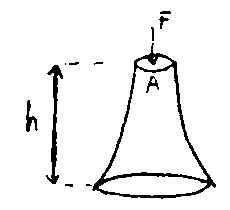
\includegraphics[width=.22\textwidth]{04_oszlop_terbeli.png}
  \hspace{1.1cm}
  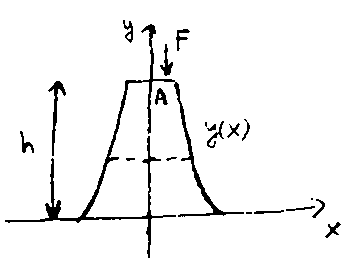
\includegraphics[width=.31\textwidth]{05_oszlop_profil.png}
\end{center}

A feltétel: minden keresztmetszetben a nyomás, azaz $F/A$
ugyanakkora legyen. A keresett $y(x)$-re elsőrendű
differenciálegyenlet adódik.

\noindent\textit{Analízis alkalmazásai,
13. oldal (feladat), 53. oldal (megoldás).}

\section{A differenciálegyenlet-rendszer és a kezdetiérték-probléma fogalma}

\subsection{A differenciálegyenlet-rendszer fogalma}

\noindent\textbf{Adott:}
\begin{itemize}
 \item $n\in\mathbb{N}$, $n>0$;
 \item $f\colon D\to\mathbb{R}^n$, $f\in C$ (folytonos);
 \item $D\subseteq\mathbb{R}\times\mathbb{R}^n$ tartomány,
       azaz összefüggő, nyílt halmaz.
\end{itemize}

\noindent\textbf{Keresünk} egy $I\subseteq\mathbb{R}$ nyílt intervallumot
és egy deriválható $\varphi\colon I\to\mathbb{R}^n$ függvényt, melyre
\begin{align*}
 (t,\varphi(t))&\in D_f &&\forall\,\text{minden } t\in I \text{ esetén},\\
 \varphi'(t)&=f\bigl(t,\varphi(t)\bigr)
     &&\forall\,\text{minden } t\in I \text{ esetén}.
\end{align*}

A fenti feladatot \textbf{elsőrendű, közönséges, explicit
differenciálegyenlet-rendszernek} (röviden: differenciálegyenletnek) nevezzük.
Az elsőrendű azt jelenti, hogy első derivált szerepel; a közönséges azt,
hogy egy független változó van; az explicit azt, hogy a keresett függvény
deriváltja ki van fejezve.

Az ilyen $\varphi$ a differenciálegyenlet \textbf{megoldása} az $I$ intervallumon.

\noindent\textbf{Jelölés:}
\[
  x'(t)=f\bigl(t,x(t)\bigr)
  \qquad\text{vagy}\qquad
  x'=f\circ(\operatorname{id},x),
  \quad \operatorname{id}(t)=t.
\]
Az $f$ függvény a differenciálegyenlet \emph{jobb oldala}.

\noindent\textbf{Szemléltetés ($n=1$):} az $f(u,v)$ értéke
meredekséget ad meg az $(u,v)$ pontban. Így minden ponthoz
meg van szabva az érintő iránya: ez az \textbf{iránymező}.
Olyan függvényt keresünk, amely illeszkedik az iránymezőhöz.

\begin{center}
  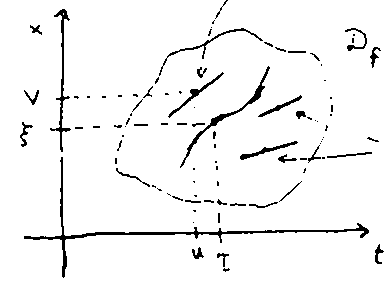
\includegraphics[width=.38\textwidth]{06_iranymezo.png}
\end{center}

\subsection{A kezdetiérték-probléma fogalma}

Adott $(\tau,\xi)\in D_f\subseteq\mathbb{R}\times\mathbb{R}^n$,
ahol $\tau\in\mathbb{R}$ és $\xi\in\mathbb{R}^n$.
A $(\tau,\xi)$ ponton átmenő megoldást keresünk:
\[
 \boxed{\begin{cases}
  x'=f\circ(\operatorname{id},x),\\
  x(\tau)=\xi.
 \end{cases}}
\]
Ez a \textbf{kezdetiérték-probléma} (k.é.p.).

\subsection{A kezdetiérték-problémára vonatkozó kérdések}

\begin{enumerate}
  \item A megoldás \textbf{létezése} (egzisztencia).
  \item A megoldás \textbf{egyértelműsége} (unicitás).
  \item A megoldások \textbf{folytathatósága}.
  \item A megoldás \textbf{előállítása}: pontosan (a félév anyaga,
        csak speciális esetekben), illetve numerikusan.
  \item A megoldások \textbf{függése a kezdeti értéktől
        és a paraméterektől}.
\end{enumerate}

\begin{center}
  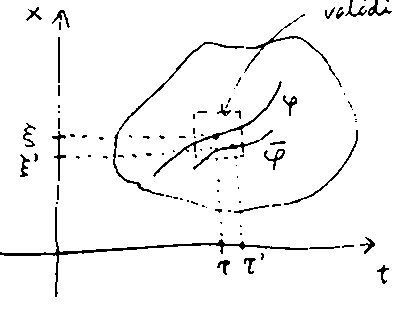
\includegraphics[width=.39\textwidth]{07_kezdeti_ertek.png}
\end{center}

Ha $(\tau',\xi')\sim(\tau,\xi)$, azaz a kezdeti értékek
közel vannak egymáshoz, mit mondhatunk a $(\tau',\xi')$-ből
induló $\overline\varphi$ megoldásról?

\noindent\textbf{Előzetes válasz:}
\begin{itemize}
  \item Adott \textbf{korlátos intervallumon}:
        $\overline\varphi\sim\varphi$.
  \item \textbf{Nem korlátos intervallumon}:
        a stabilitáselmélet kérdéseihez jutunk.
\end{itemize}

Például: $x'=\alpha x$.

\begin{center}
  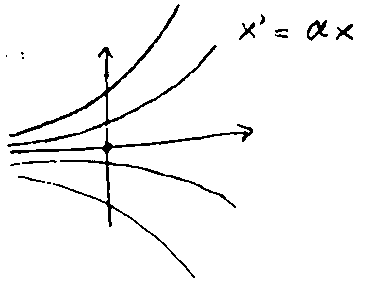
\includegraphics[width=.31\textwidth]{08_alpha_x.png}
\end{center}

\noindent\textbf{6. Minőségi vizsgálatok:} a megoldások bizonyos
tulajdonságainak vizsgálata. (például a megoldás pozitivitása, vagy periodicitása)
